\section*{Appendix A - Ábrák} \label{A}
\topskip0pt
\vspace*{\fill}
\begin{center}
    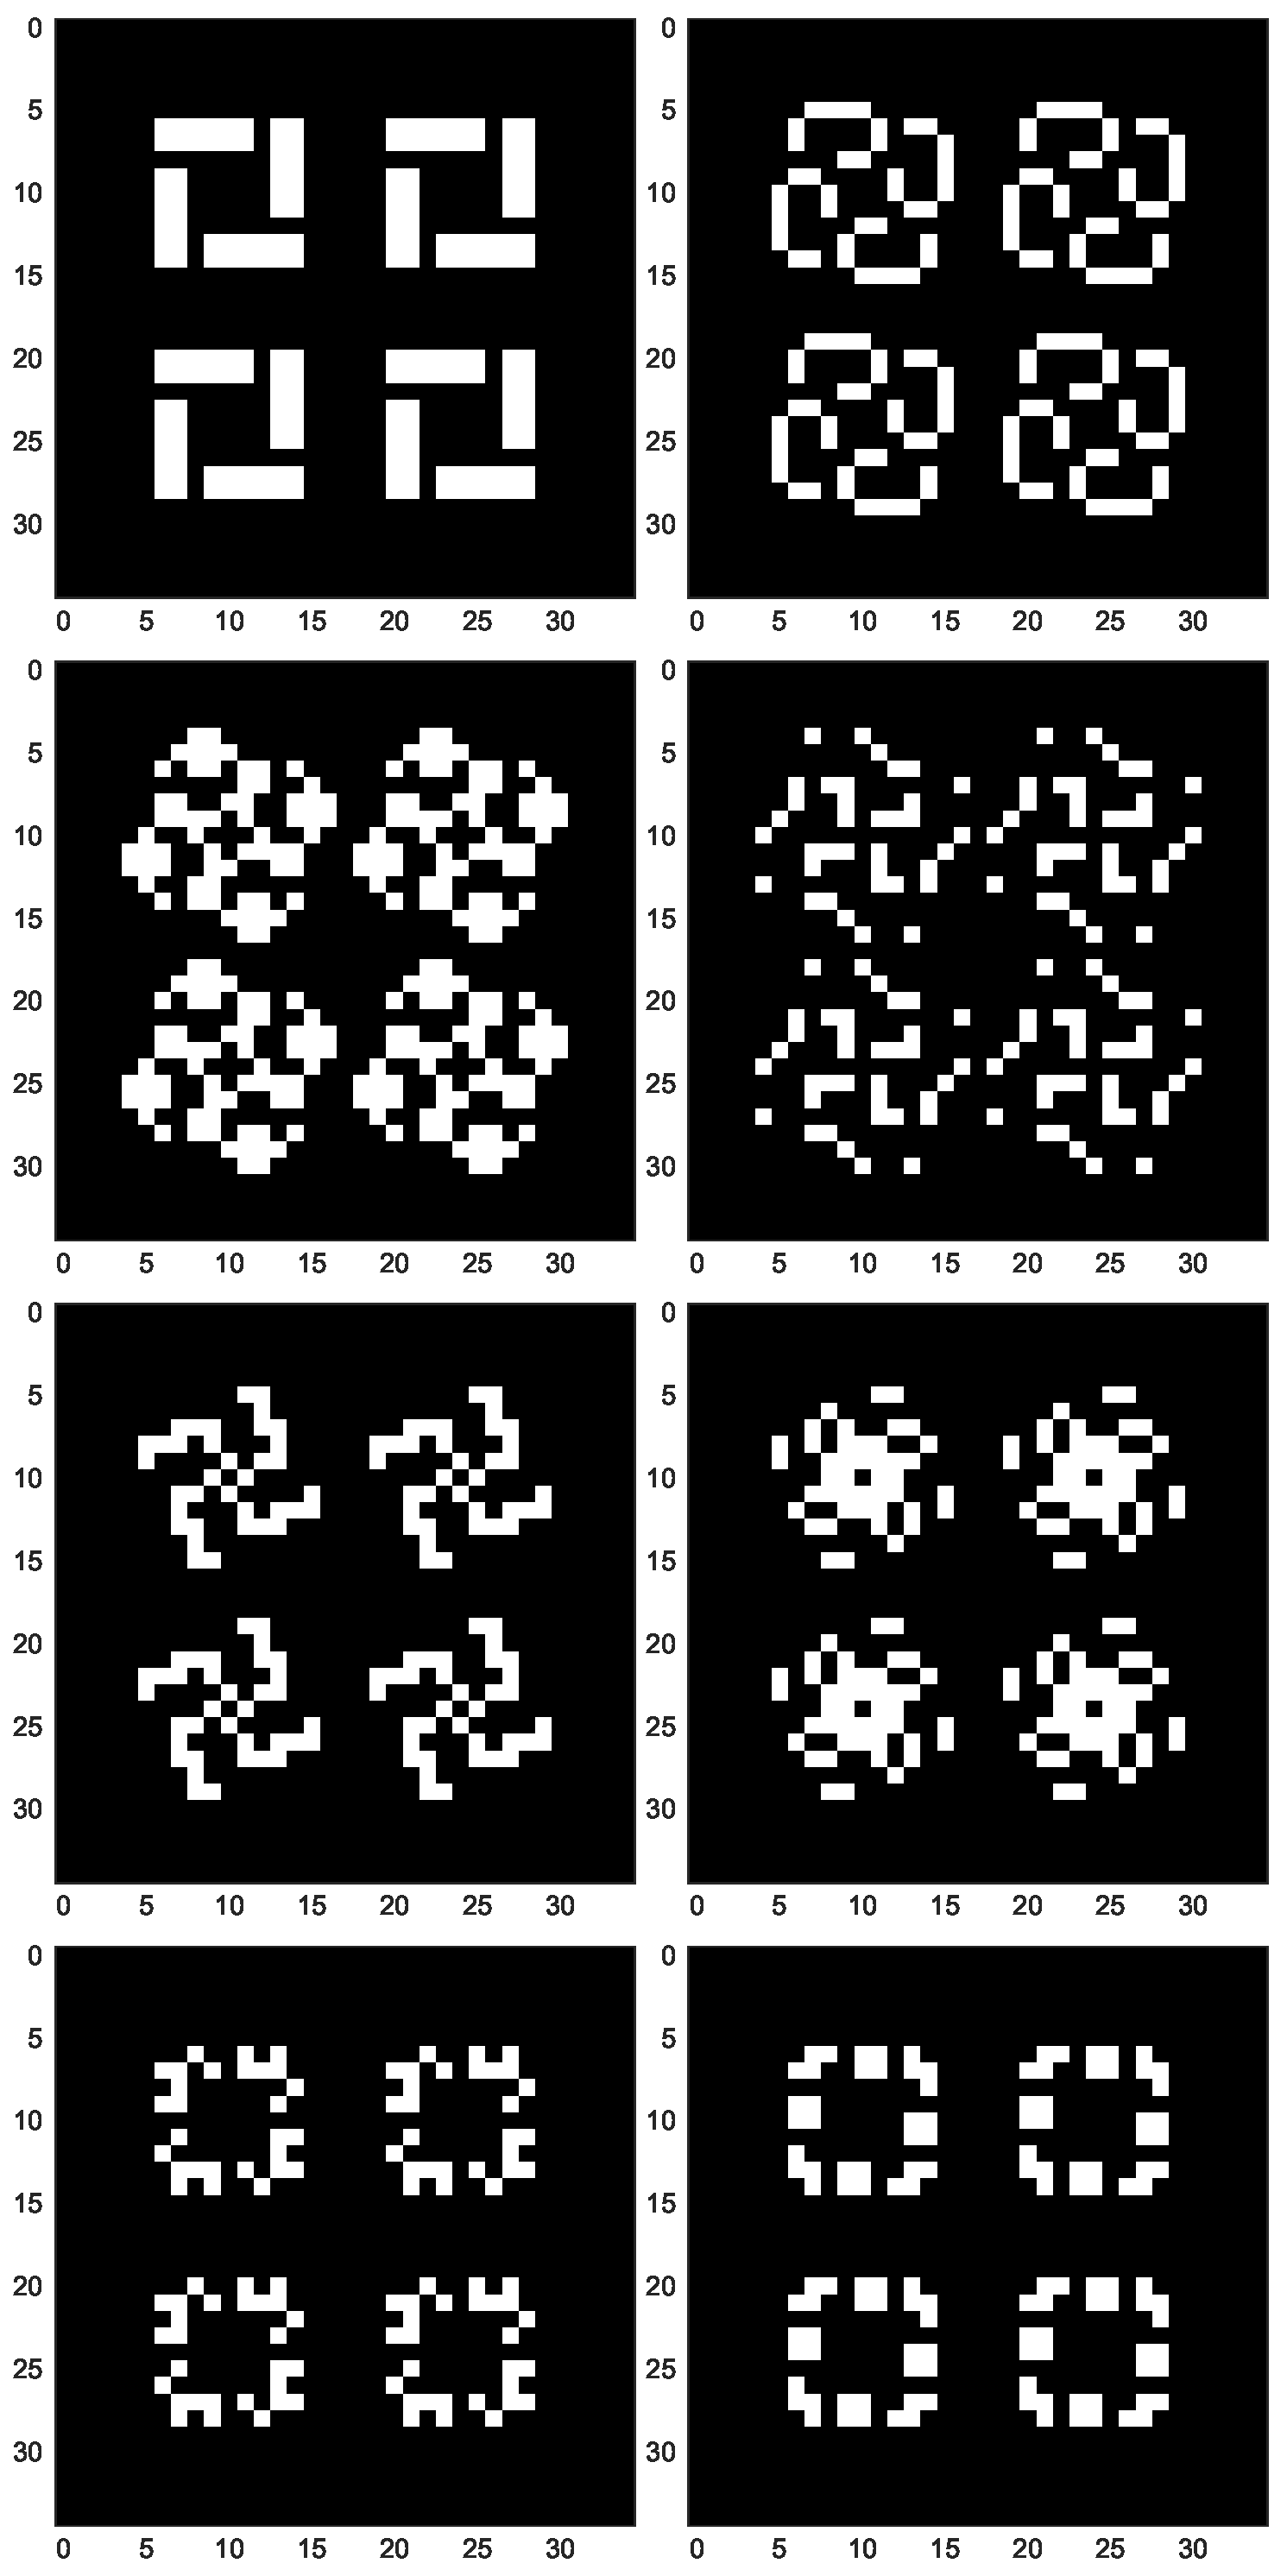
\includegraphics[width=0.8\textwidth]{images/galaxy.pdf}
    \captionof{figure}{A Conway-féle Életjáték egyik oszcillátora, a \emph{Kok's galaxy}. A játék ebben az esetben a standard, $N=3$ szabályt használja. A rendszer egy nyolc-állapotú oszcillátor, mely egy galaxis-szerű forgást imitál.} \label{fig:1}
\end{center}
\vspace*{\fill}
\newpage
\topskip0pt
\vspace*{\fill}
\begin{center}
    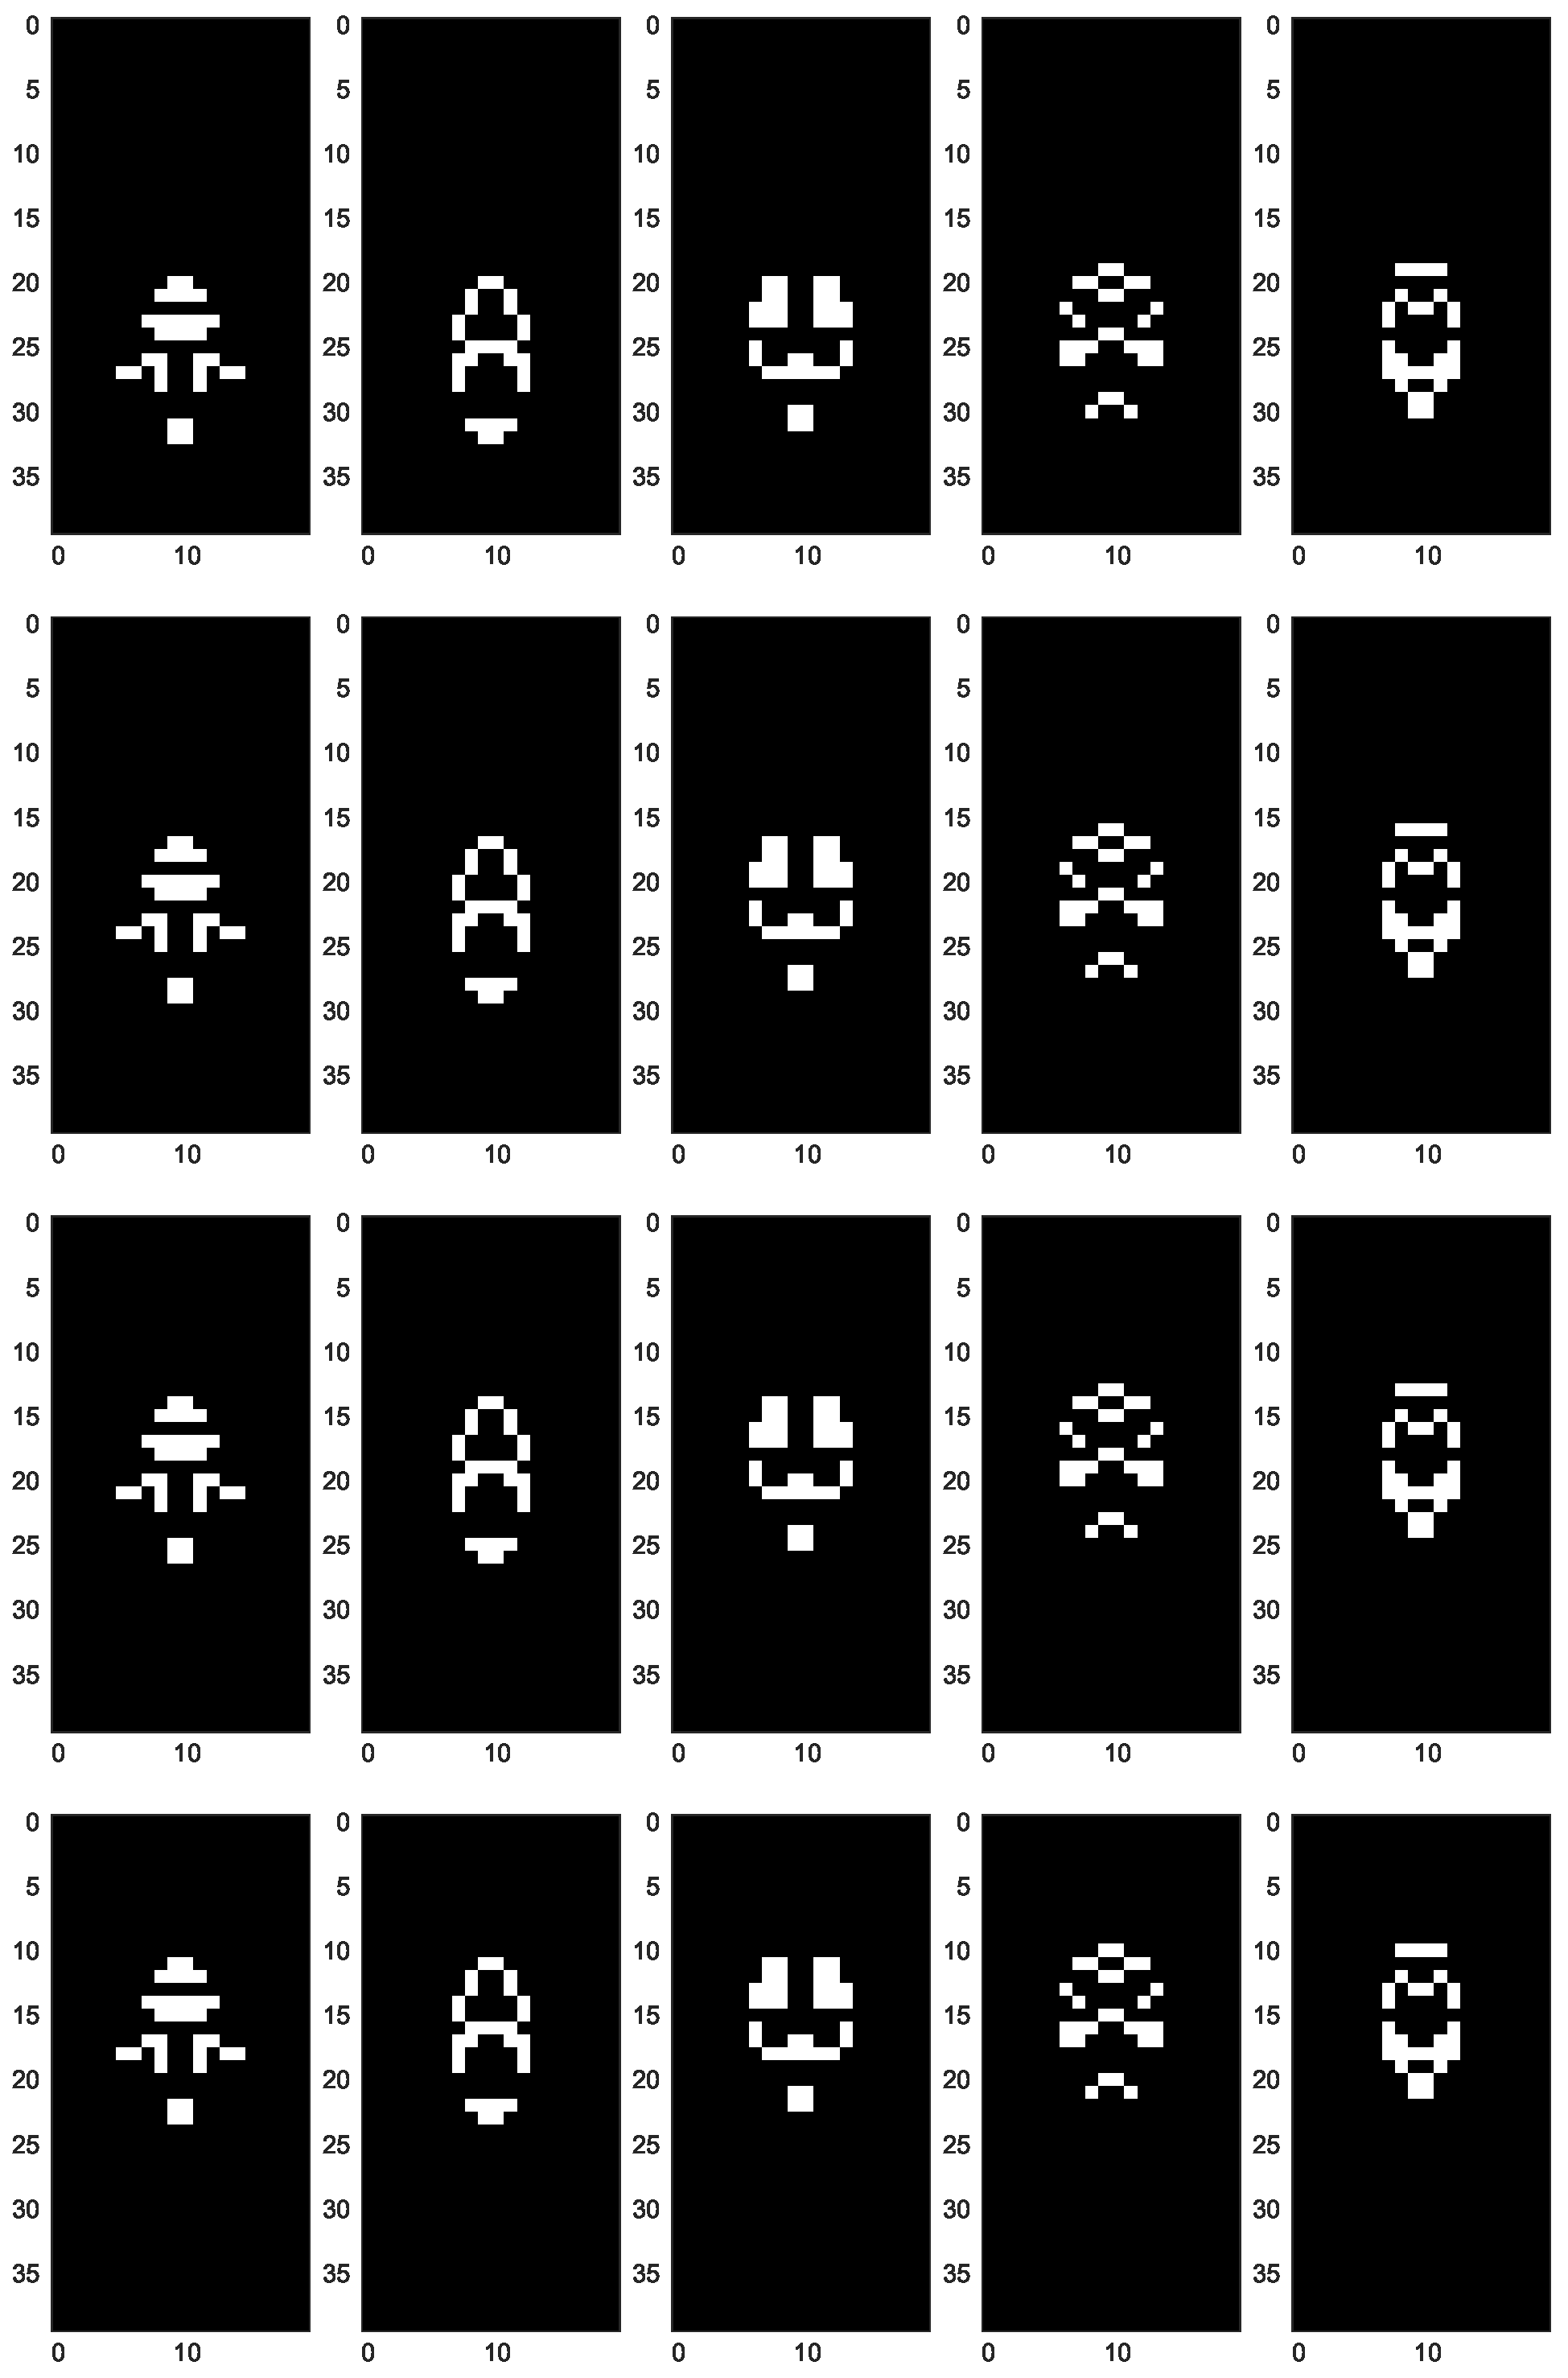
\includegraphics[width=\textwidth]{images/copperhead.pdf}
    \captionof{figure}{A Conway-féle Életjáték egyik űrhajója, a \emph{Copperhead}. A játék ebben az esetben a standard, $N=3$ szabályt használja. A Copperhead űrhajó $c/10$ sebességgel halad folyamatosan felfelé a játékmezőn. Az ábrán csak minden 6. lépés illusztráltam, hogy mozgásának iránya látható legyen.} \label{fig:2}
\end{center}
\vspace*{\fill}
\newpage
\topskip0pt
\vspace*{\fill}
\begin{center}
    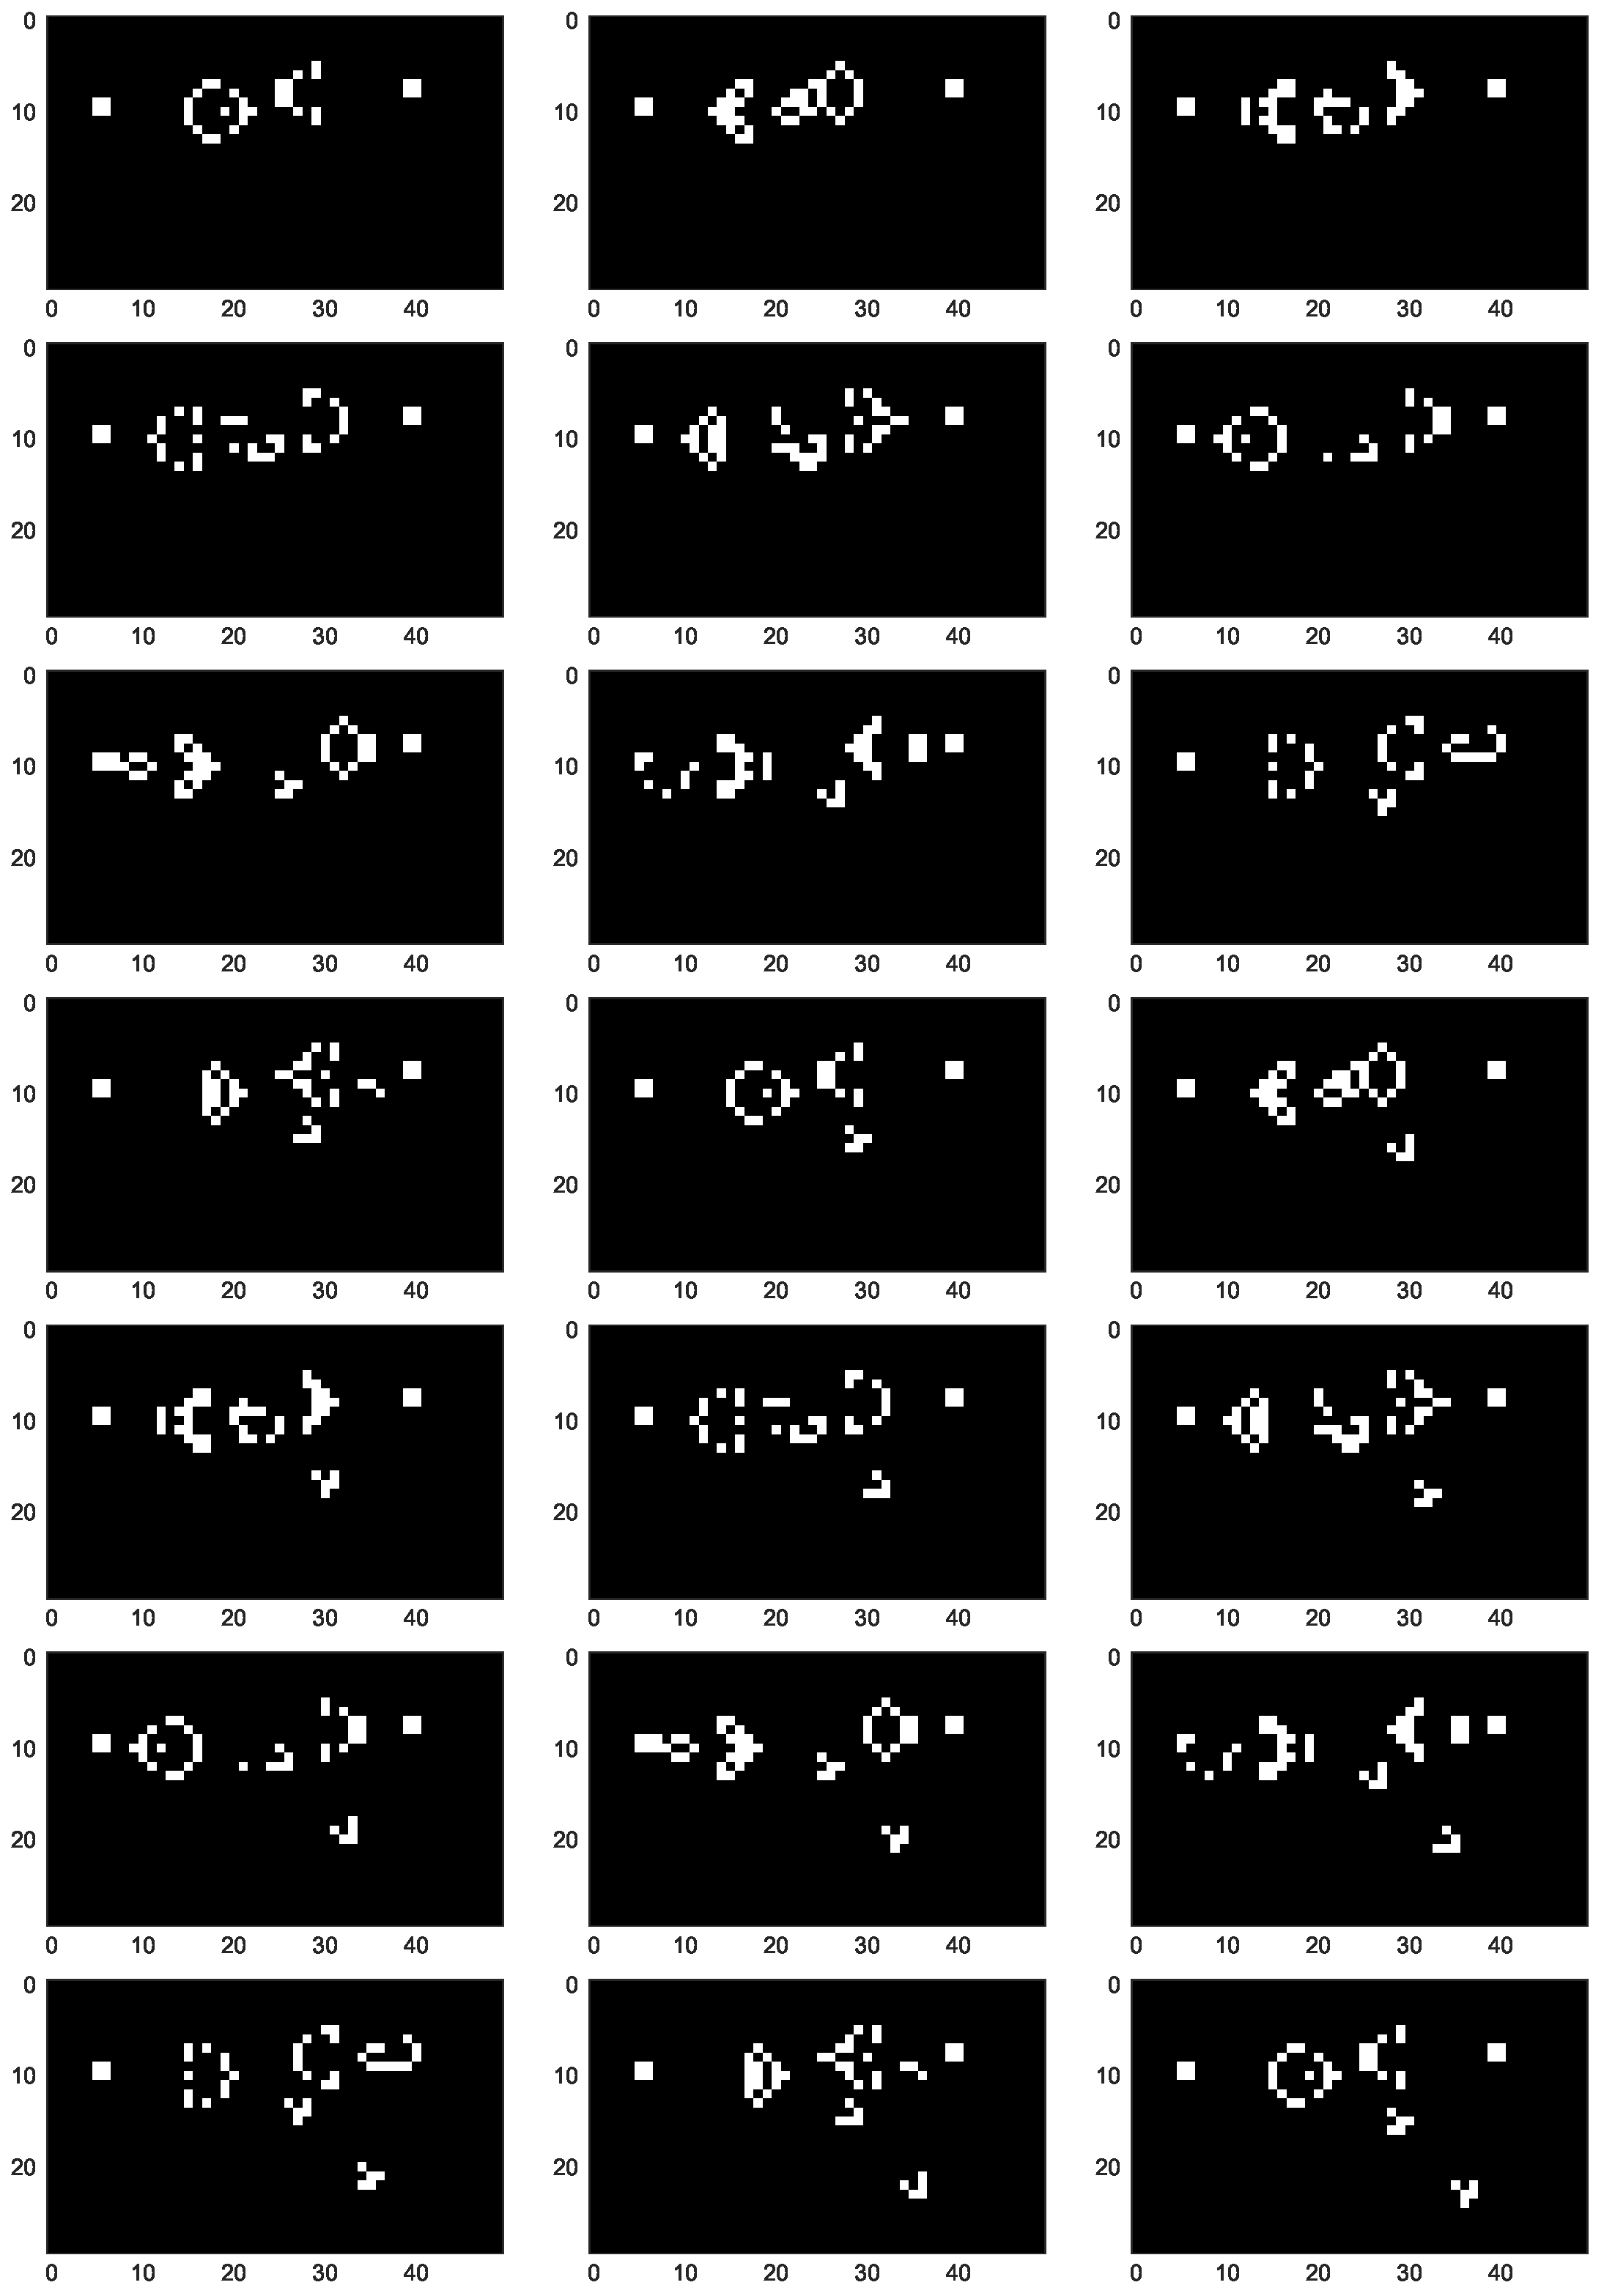
\includegraphics[width=\textwidth]{images/glidergun.pdf}
    \captionof{figure}{A Conway-féle Életjáték egyik \emph{gun}-ja, a \emph{Gosper glider gun}. A játék ebben az esetben a standard, $N=3$ szabályt használja. A legelső ismert \emph{gun} valójában két darab, egy-egy blokkal stabilizált \emph{Queen bee shuttle}, melyek így minden periódusukban kibocsájtani egy $c/4$ sebességgel, diagonálisan haladó \emph{Glider}t. Az ábrán csak minden 3. lépés illusztráltam, hogy a Gliderek kilövése és a forma oszcillációja jól látható legyen.} \label{fig:3}
\end{center}
\vspace*{\fill}
\newpage
\topskip0pt
\vspace*{\fill}
\begin{center}
    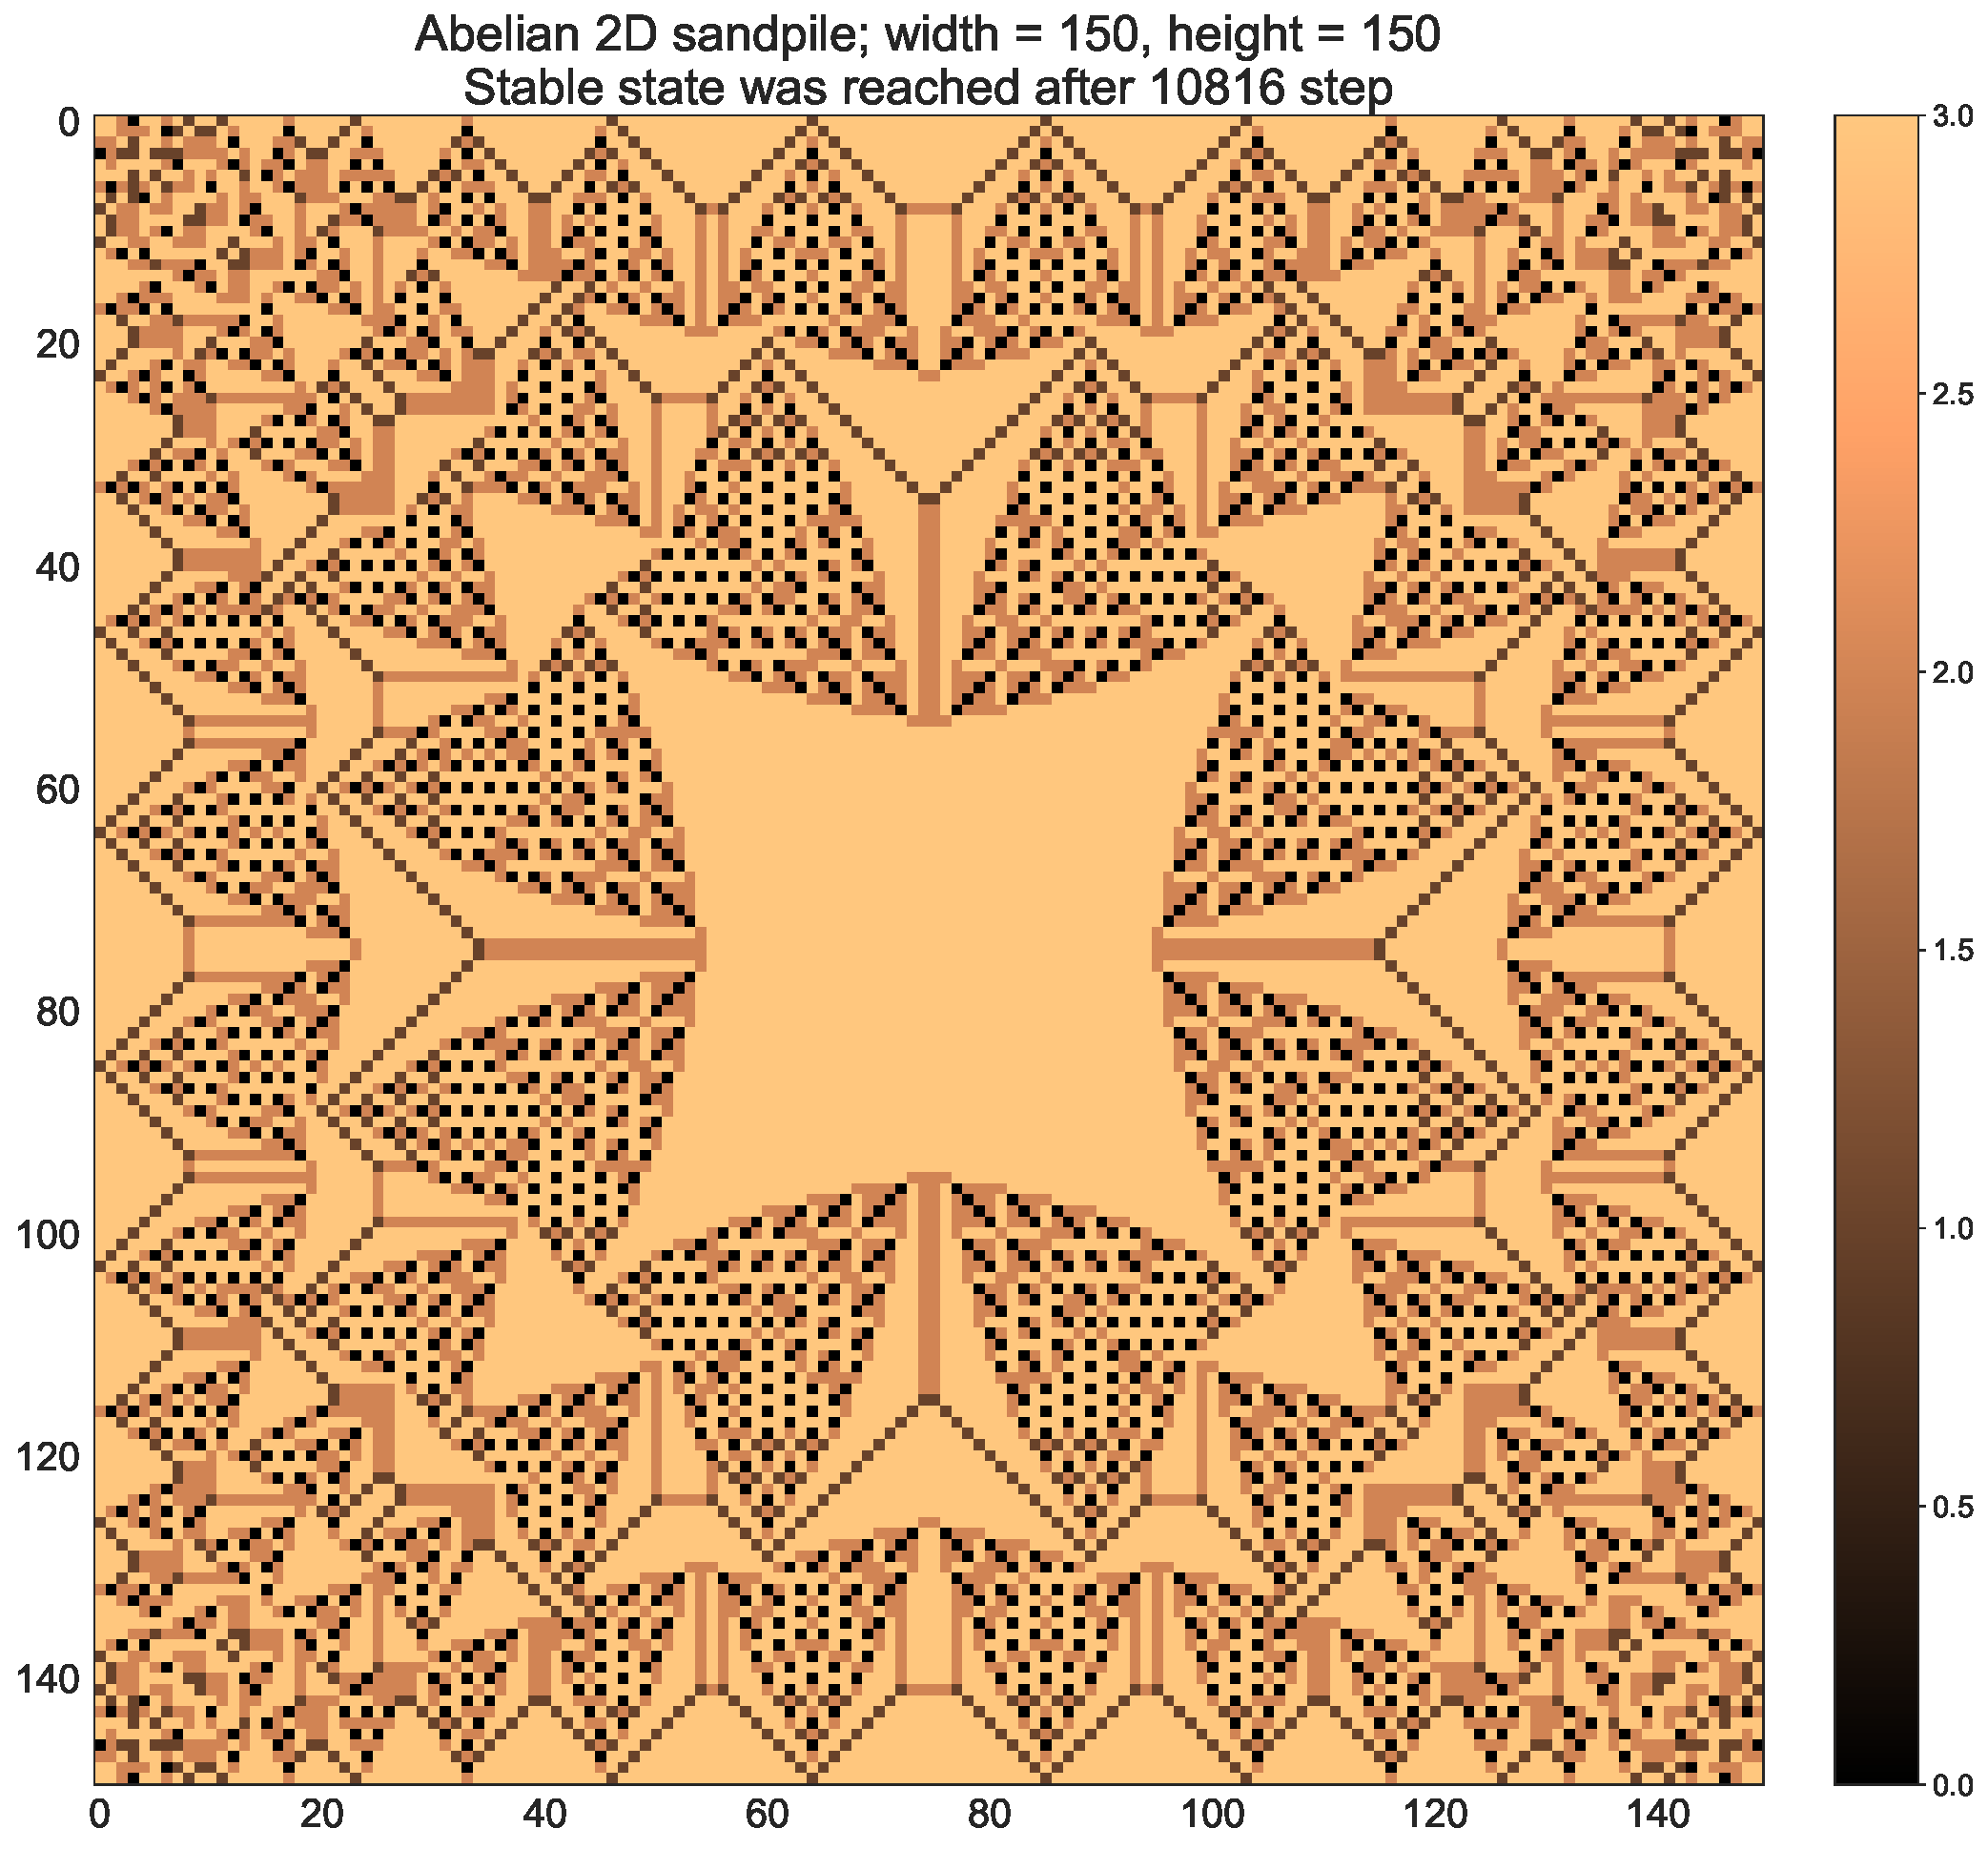
\includegraphics[width=0.87\textwidth]{images/sandpile_w150_h150.pdf}
    \captionof{figure}{Az Abel-féle 2D homokdomb modell stabil állapota $150 \times 150$ nagyságú területre, $s = 7$ maximális toronymagasság esetén.} \label{fig:4}
\end{center}
\begin{center}
    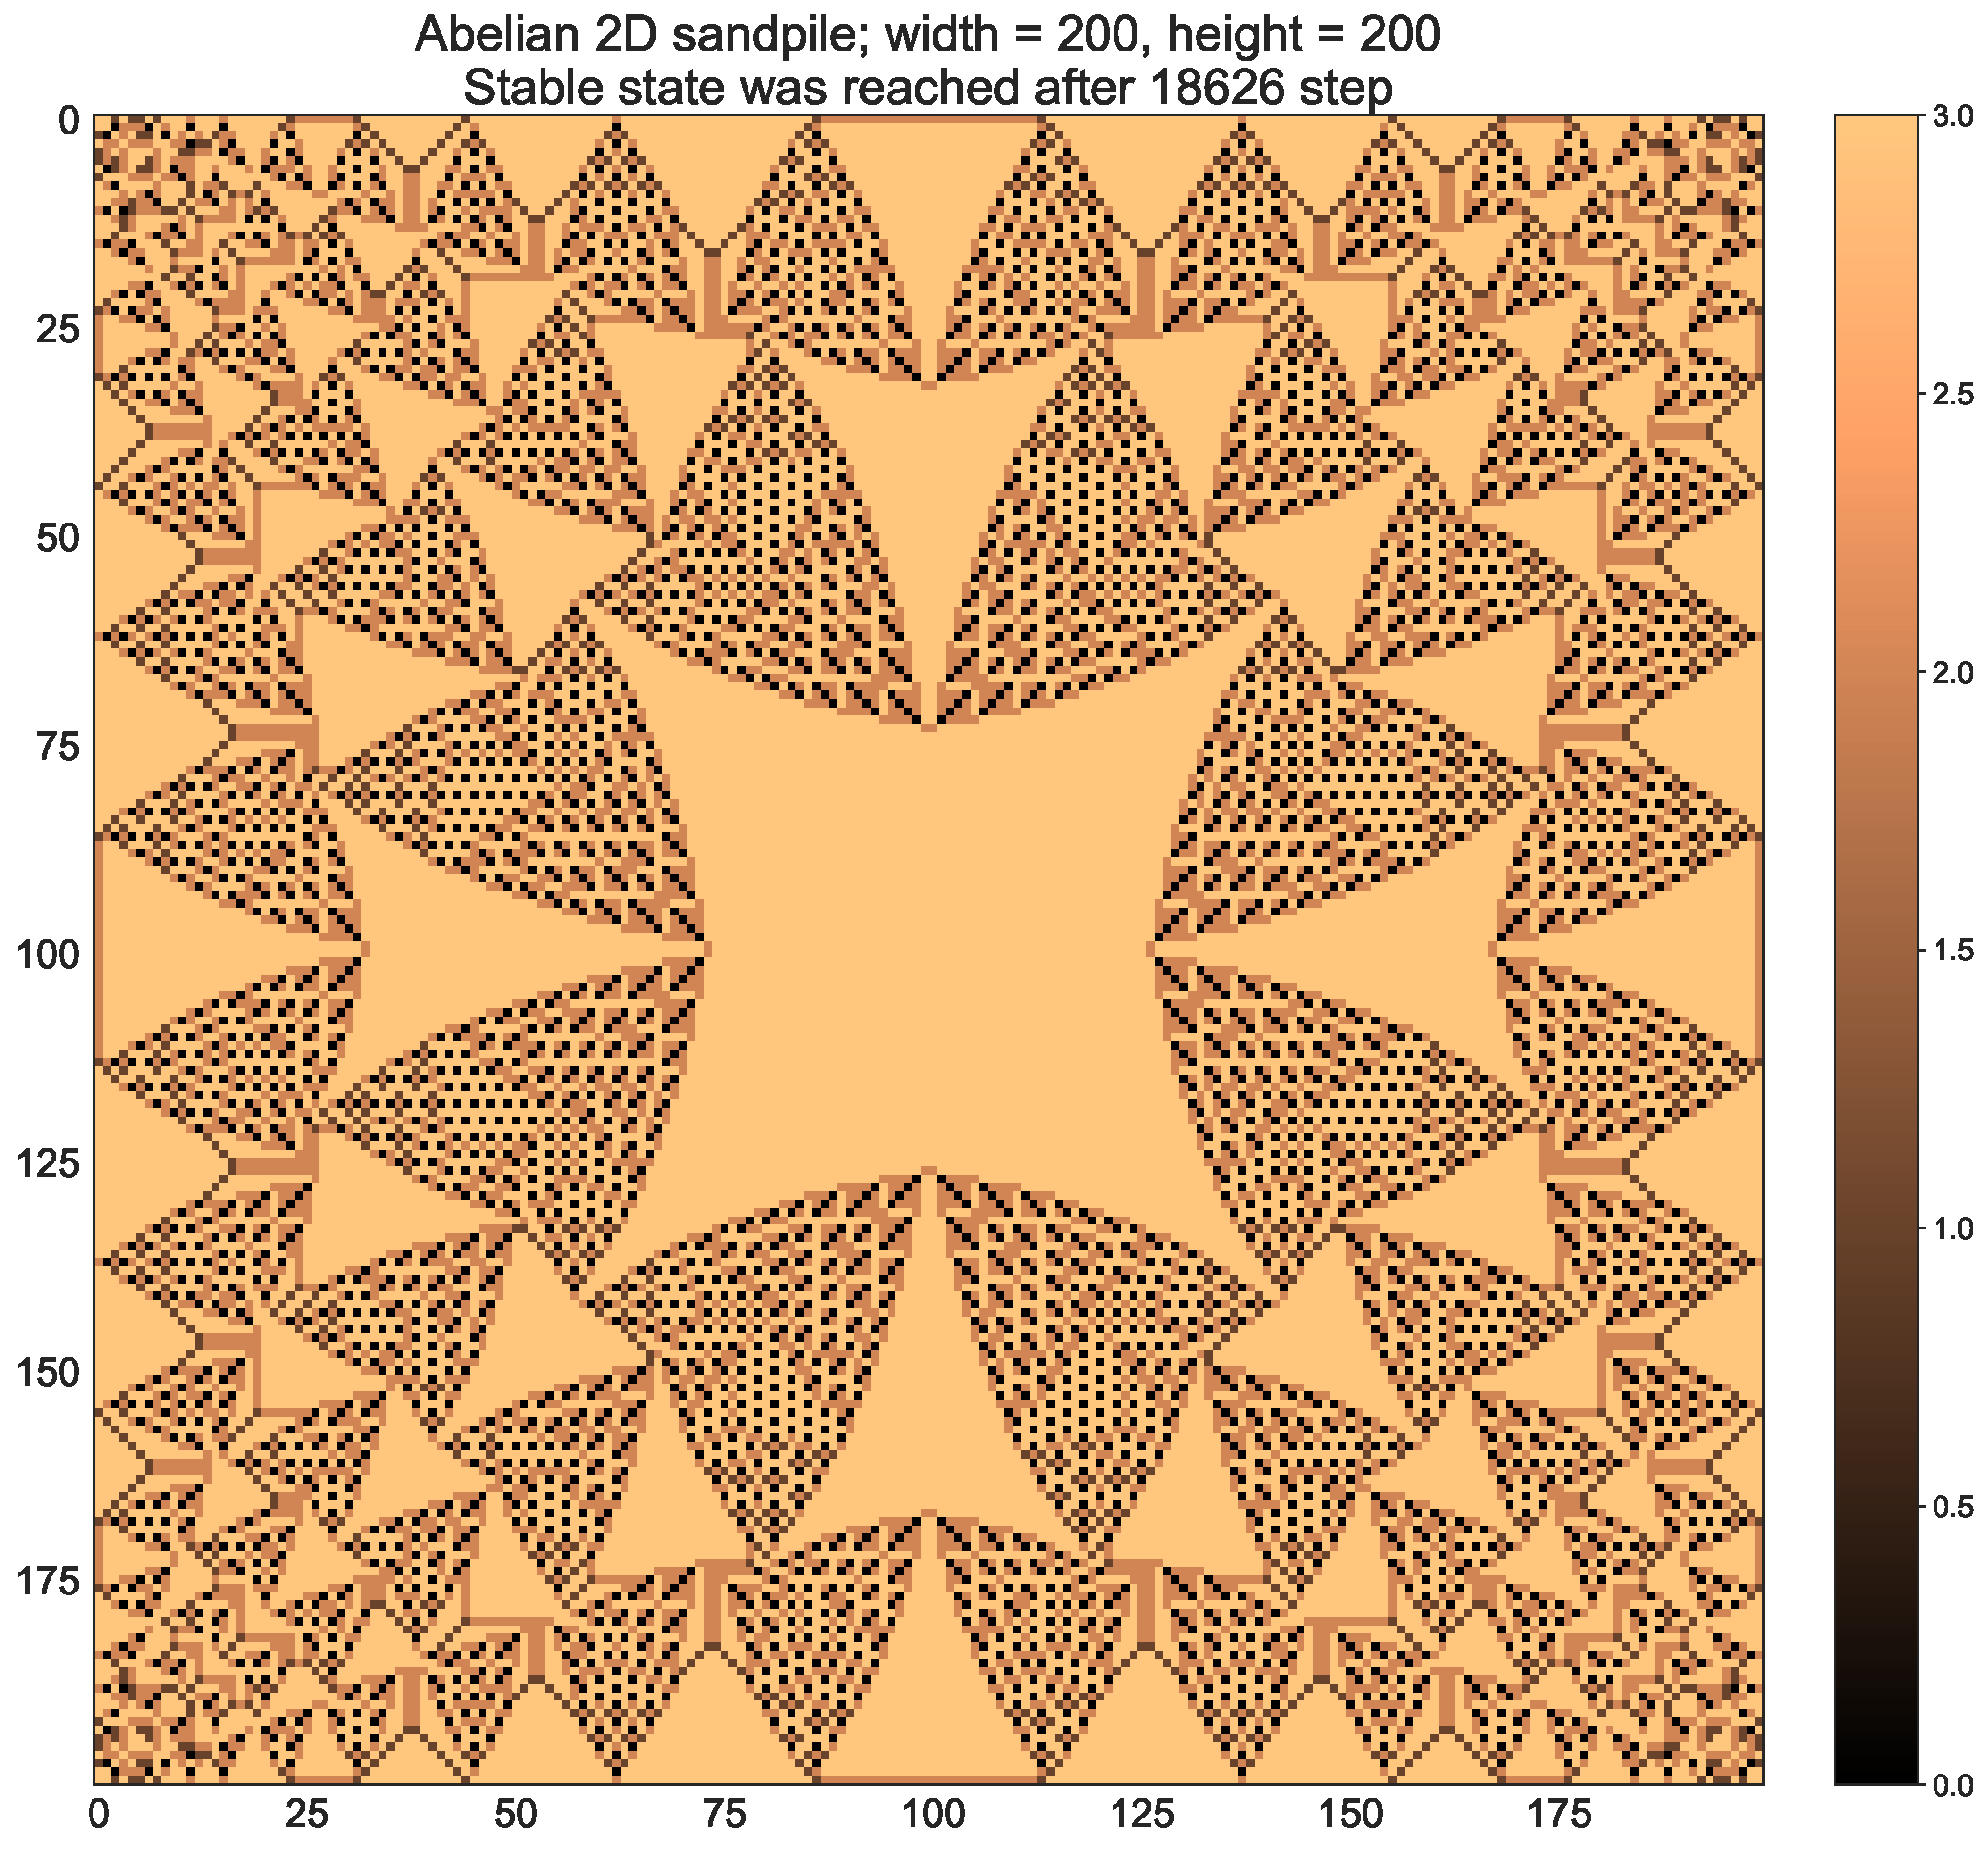
\includegraphics[width=0.87\textwidth]{images/sandpile_w200_h200.pdf}
    \captionof{figure}{Az Abel-féle 2D homokdomb modell stabil állapota $200 \times 200$ nagyságú területre, $s = 7$ maximális toronymagasság esetén.} \label{fig:5}
\end{center}
\vspace*{\fill}
\newpage
\topskip0pt
\vspace*{\fill}
\begin{center}
    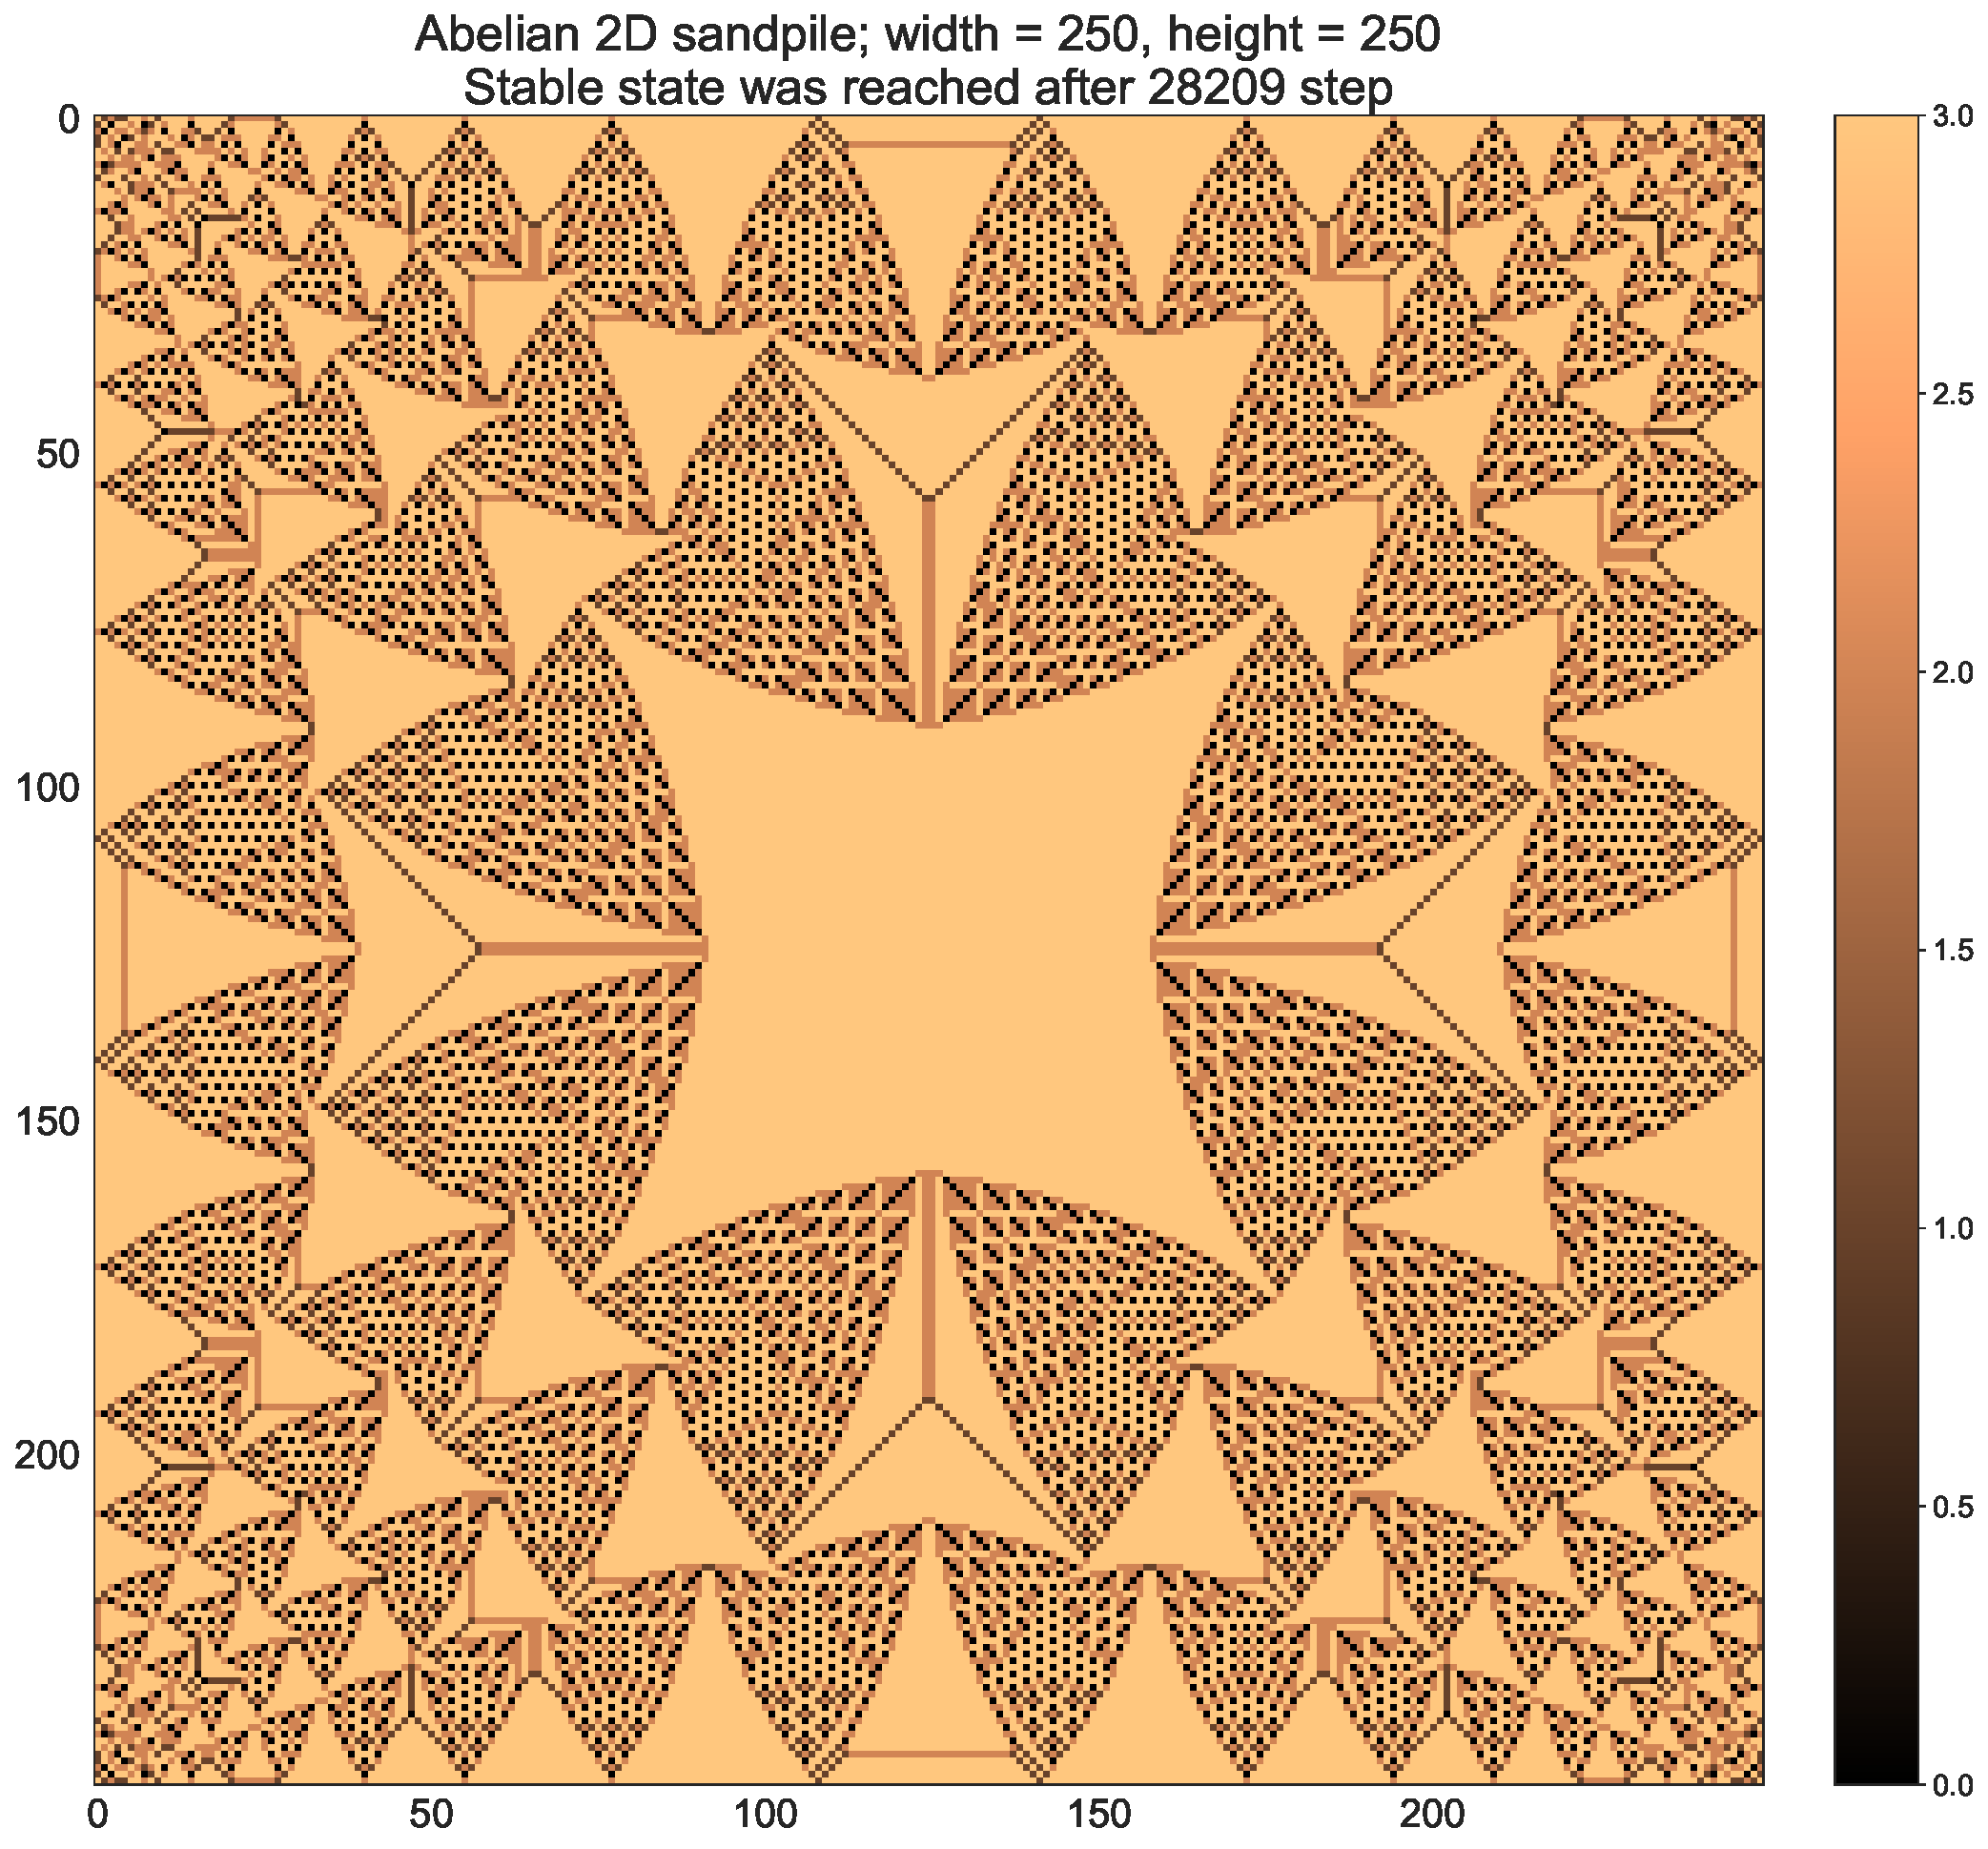
\includegraphics[width=0.87\textwidth]{images/sandpile_w250_h250.pdf}
    \captionof{figure}{Az Abel-féle 2D homokdomb modell stabil állapota $250 \times 250$ nagyságú területre, $s = 7$ maximális toronymagasság esetén.} \label{fig:6}
\end{center}
\begin{center}
    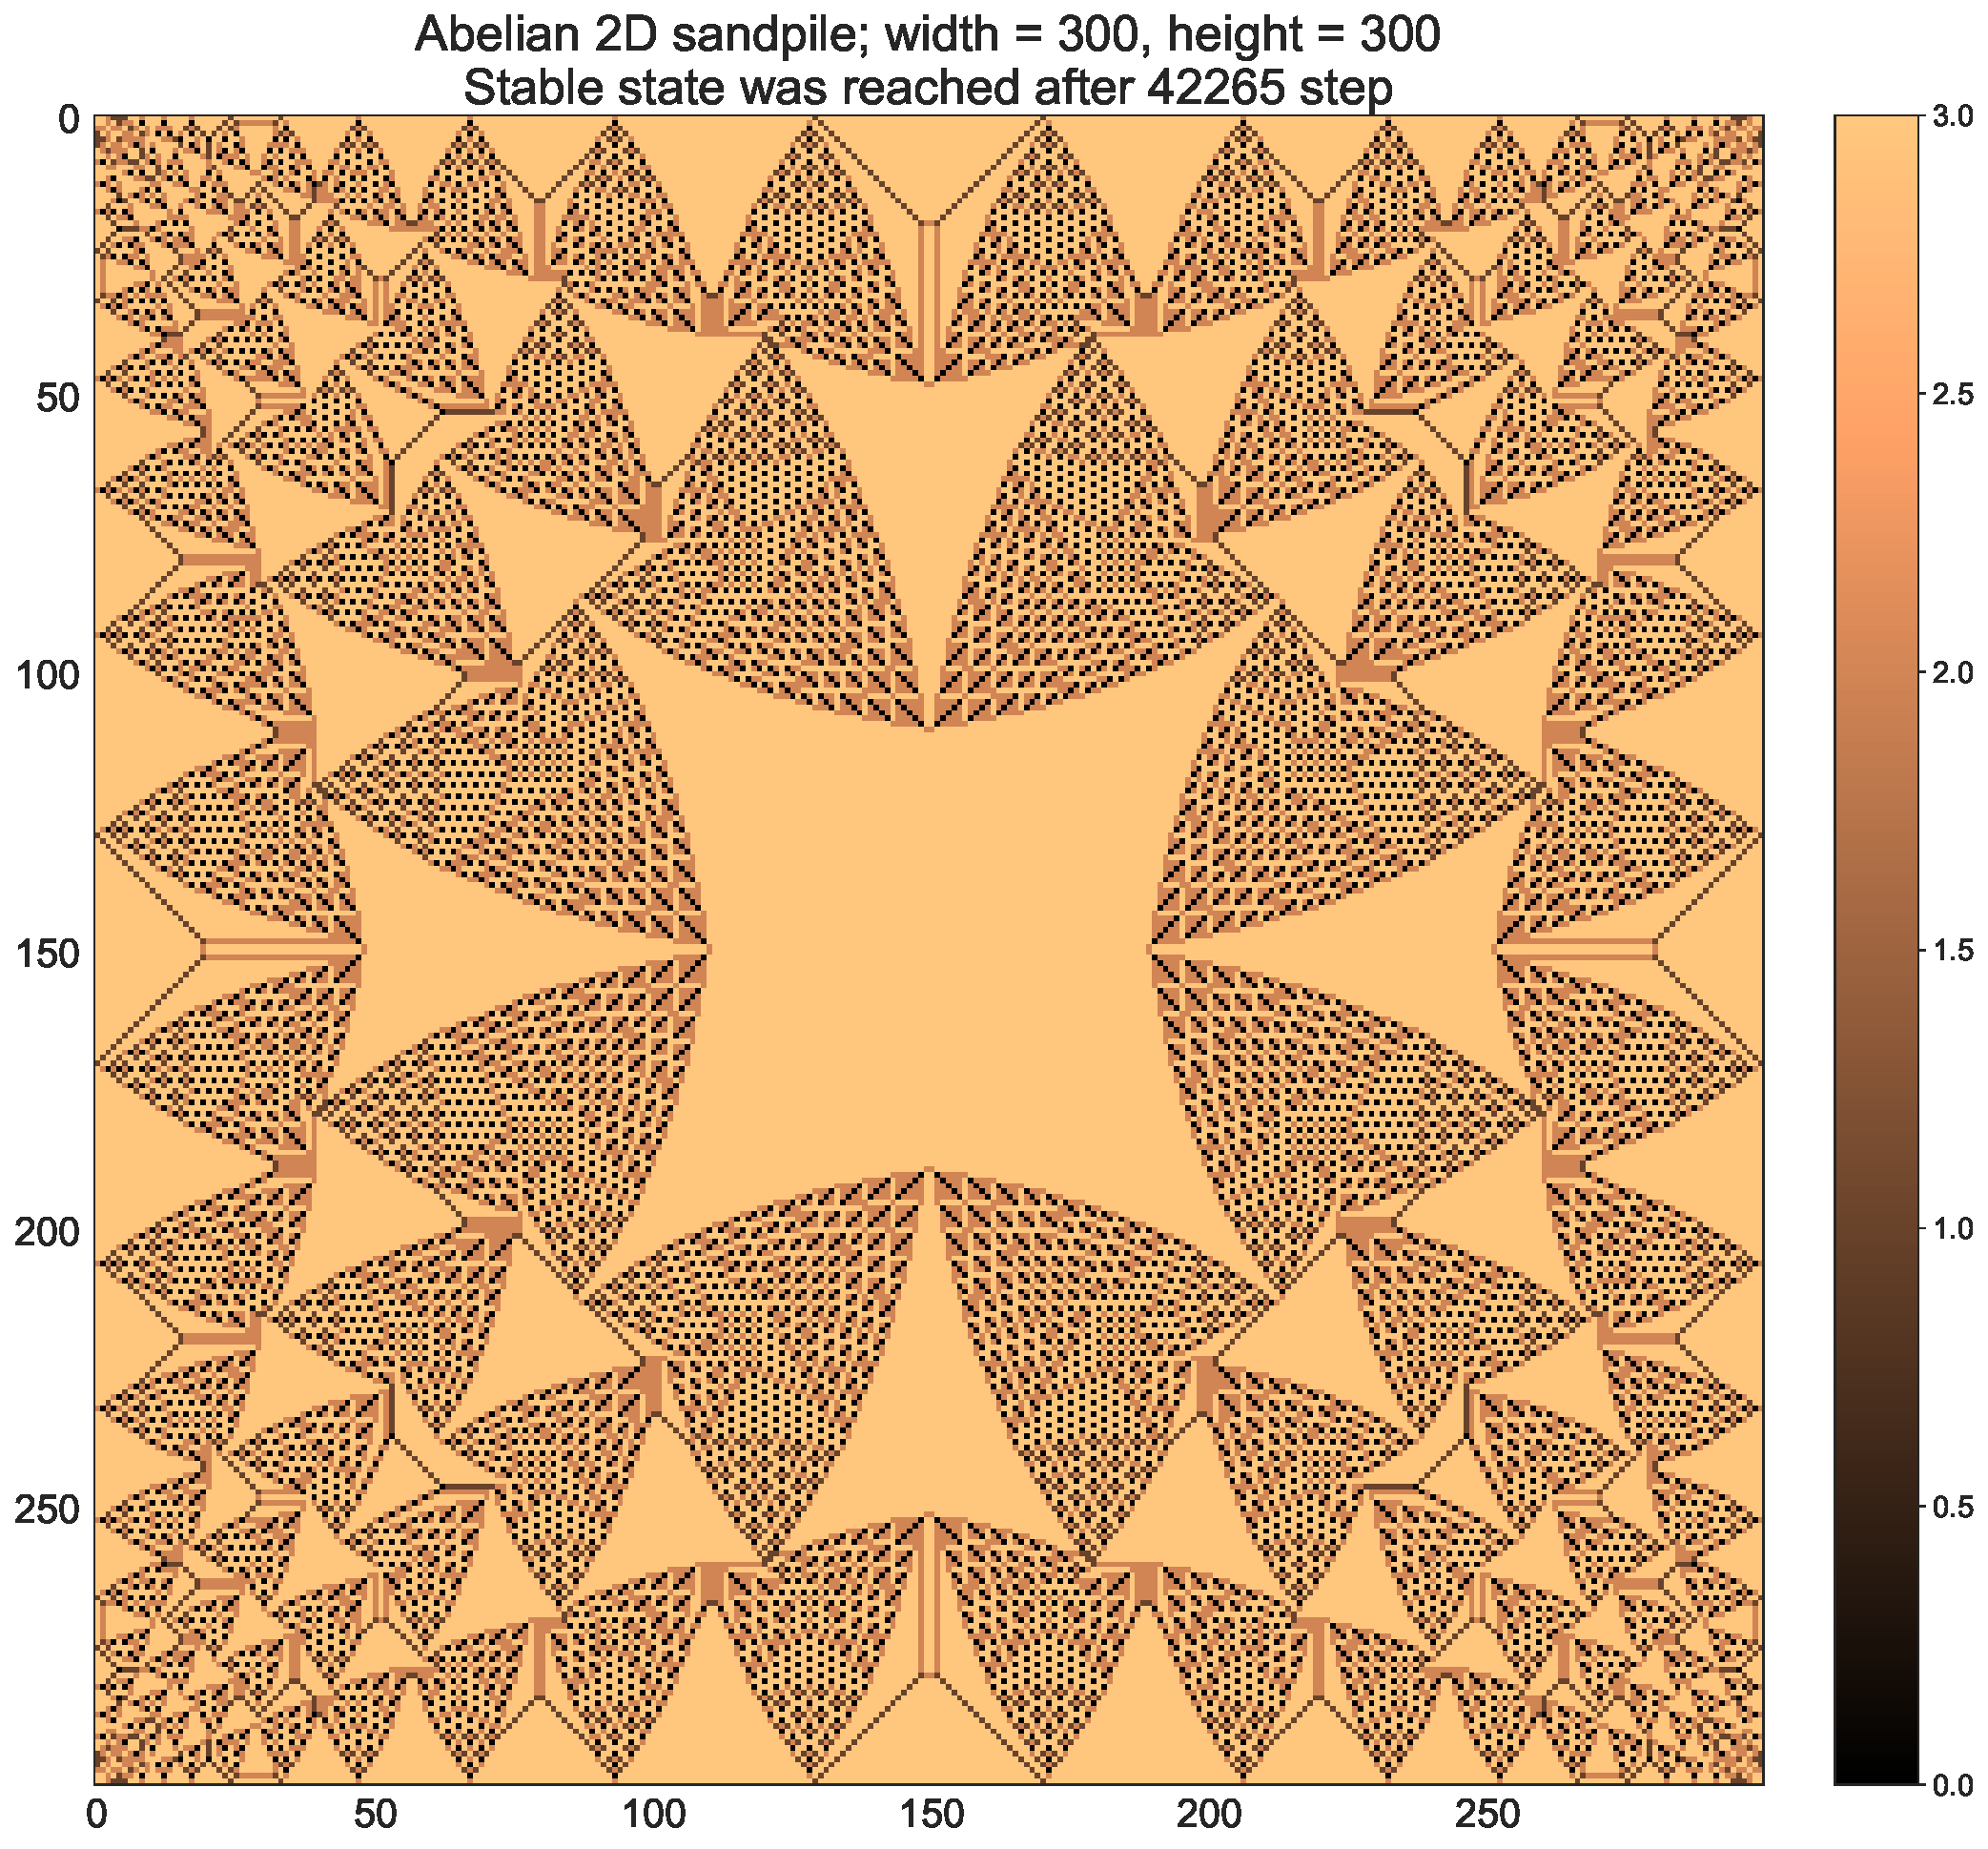
\includegraphics[width=0.87\textwidth]{images/sandpile_w300_h300.pdf}
    \captionof{figure}{Az Abel-féle 2D homokdomb modell stabil állapota $300 \times 300$ nagyságú területre, $s = 7$ maximális toronymagasság esetén.} \label{fig:7}
\end{center}
\vspace*{\fill}